\subsection{Funktionsweise}
\label{subsec:cdfunktionsweise}

Die Compact Disc besteht aus einer Polycarbonatscheibe und einer 40-80nm dicken
zumeist aus Aluminium bestehenden Reflexionsschicht. Zusätzlich gibt es noch
eine 10-20µm dicke Lackschicht welche die Reflexionsschicht schützt.
Zusammengenommen ergibt dies eine Höhe von ca. 1,2mm wie man in
\autoref{fig:cdquer} erkennen kann. Außerdem lässt sich eine
Einbuchtung(\textit{pit}), welche sich von der Grundebene(\textit{land}) abhebt,
erkennen. \cite{cfcd}

\begin{figure}[h]
  \begin{center}
      \begin{minipage}[t]{\textwidth}
        \begin{center}
            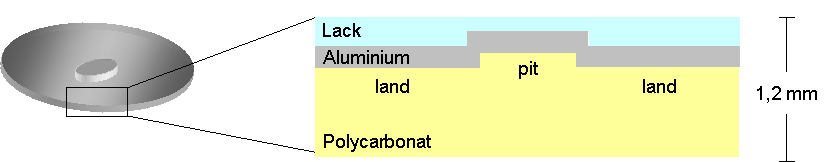
\includegraphics[height=0.1\textheight]{Bilder/Optische_Datentraeger_Die_Compact_Disc/Funktionsweise/cdquer.png}
            \caption[Querschnitt einer CD (Skizze) \newline \url{http://daten.didaktikchemie.uni-bayreuth.de/umat/cd_dvd/cd_dvd.htm} (zuletzt aufgerufen am 07.08.2015)]{Querschnitt einer CD (Skizze)}
            \label{fig:cdquer}
        \end{center}
      \end{minipage}
  \end{center}
\end{figure}

Die Abtasteinheit, welche aus einem Laser und einem Fotodetektor besteht, liest
spiralförmig von innen nach außen die Informationen auf der CD aus. Dafür
wandelt der Fotodetektor das von der Reflexionsschicht zurückgeworfene
Laserlichtes in Strom um, wobei die Stromstärke abhängig von der Lichtintensität
ist. Eine Abnahme der Lichtintensität kann man beim Überstreifen des
Laserstrahls von einem \textit{pit} erkennen und resultiert in einer Abnahme der
Stromstärke. Da der Durchmesser des Laserstrahls größer ist als die Pitbreite
(siehe \autoref{fig:cdrem}) trifft dieser nur teilweise auf den \textit{pit}.
Der Rest des Lichtes trifft mit geringer Verzögerung auf den Umgebenden
\textit{land}. Die Verschiebung der Strahlen gegeneinander, welche man in
\autoref{fig:cdlaser} erkennen kann, resultiert in einer Intensitätsabnahme
bedingt durch die teilweisige Auslöschung des Laserlichtes aufgrund der
destruktiven Interferenz\footnote{Wellenberg und Wellental zweier Lichtstrahlen
mit gleicher Frequenz und Amplitude treffen aufeinander und heben sich
gegenseitig auf.}. \autoref{fig:cdstrom} zeigt einen möglichen
Stromstärkenverlauf. Die Übergänge zwischen \textit{pit} und \textit{land} wird
der Binärwert 1 zugewiesen. Dies entspricht dem Schnittpunkt zwischen dem
Mittelwert und dem Graph der Stromstärke in \autoref{fig:cdstrom}. \cite{cdp}

\begin{figure}[h]
  \begin{center}
      \begin{minipage}[t]{0.3\textwidth}
        \begin{center}
            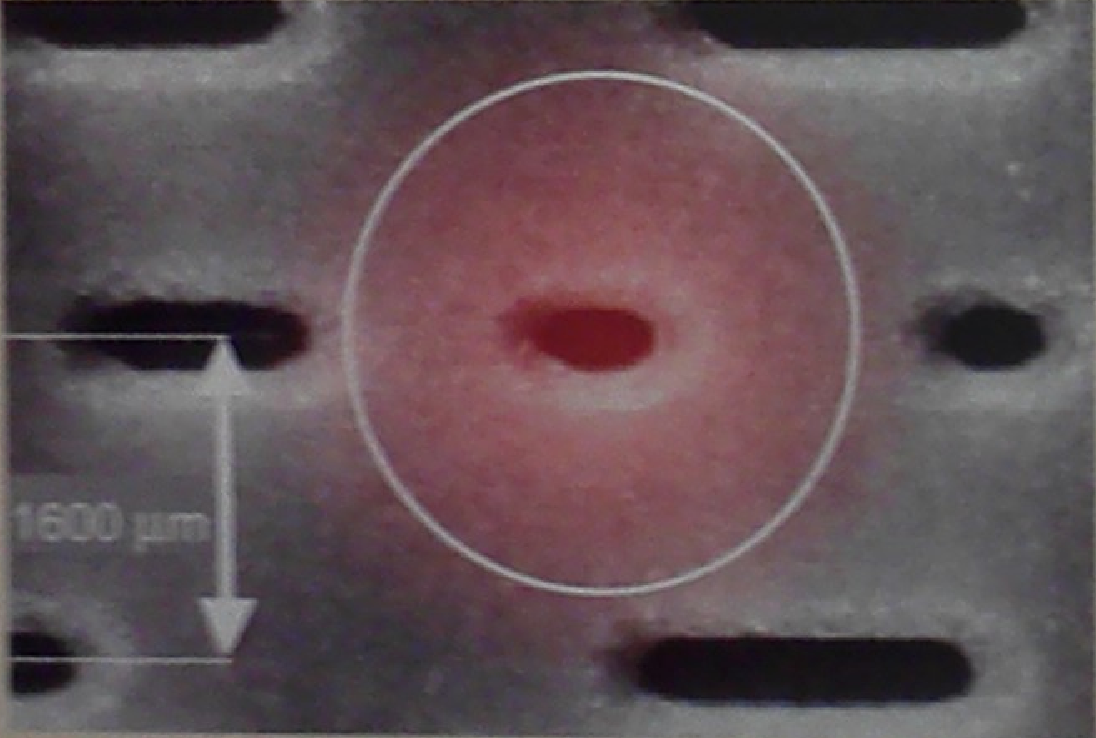
\includegraphics[height=0.1\textheight]{/home/i-bot/workspace/Seminararbeit/Bilder/Optische_Datentraeger_Die_Compact_Disc/Funktionsweise/remcd.png}
            \caption[Laserlicht auf einem \textit{pit} unter einem Rasterelektronenmikroskop \newline Roth, Klaus: CD, DVD0 \& Co.: Die Chemie der schillernden Scheiben, in: Chemie in unserer Zeit (41/2007), S. 340]{Laserlicht auf einem \textit{pit} unter einem Rasterelektronenmikroskop}
            \label{fig:cdrem}
        \end{center}
      \end{minipage}
      \hspace{0.025\textwidth}
      \begin{minipage}[t]{0.3\textwidth}
        \begin{center}
            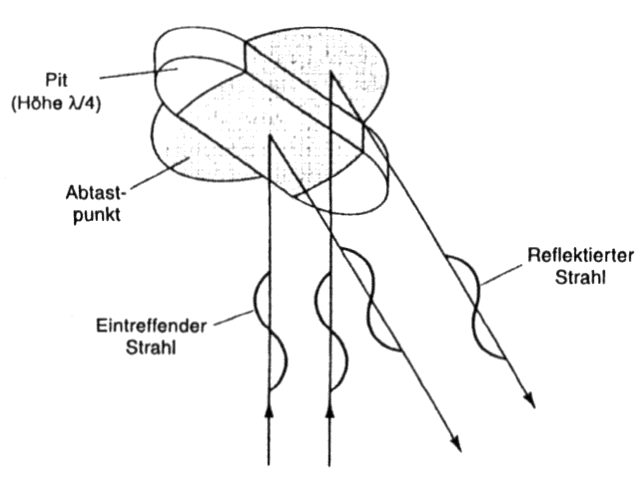
\includegraphics[height=0.1\textheight]{Bilder/Optische_Datentraeger_Die_Compact_Disc/Funktionsweise/cdlaser.png}
            \caption[destruktieve Interferenz von Laserlicht bei einem \textit{pit} (Skizze) \newline \url{http://www.muenster.de/~asshoff/physik/cd/image50.gif} (zuletzt aufgerufen am 07.08.2015)]{destruktieve Interferenz von Laserlicht bei einem \textit{pit} (Skizze)}
            \label{fig:cdlaser}
        \end{center}
      \end{minipage}
      \hspace{0.025\textwidth}
      \begin{minipage}[t]{0.3\textwidth}
        \begin{center}
            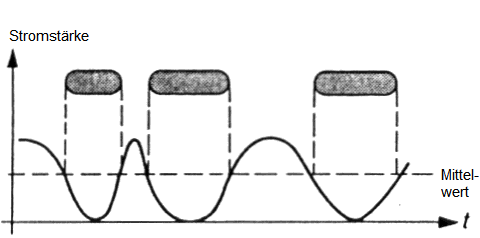
\includegraphics[height=0.09\textheight]{Bilder/Optische_Datentraeger_Die_Compact_Disc/Funktionsweise/cdstrom.png}
            \caption[Stromstärkenverlauf \newline \url{http://www.muenster.de/~asshoff/physik/cd/image51.gif} (zuletzt aufgerufen am 07.08.2015)]{Stromstärkenver-lauf}
            \label{fig:cdstrom}
        \end{center}
      \end{minipage}
  \end{center}
\end{figure}

%TODO: Referenz auf Material: Polycarbonat?
